\subsection{Data augmentation}
    
    We apply various photometric data augmentation techniques such as random hue (Fig. \ref{hue}), random brightness (Fig. \ref{brightness}), random contrast (Fig. \ref{contrast}) and random saturation (Fig. \ref{saturation}). The data augmentation techniques in Fig. \ref{photometric_data_augmentation} are applied over Fig. \ref{original}. 
    
    \def \scalevaraugmentation {0.09}
    \begin{figure}[!b] 
    \centering
    \subfloat[Original]{%
        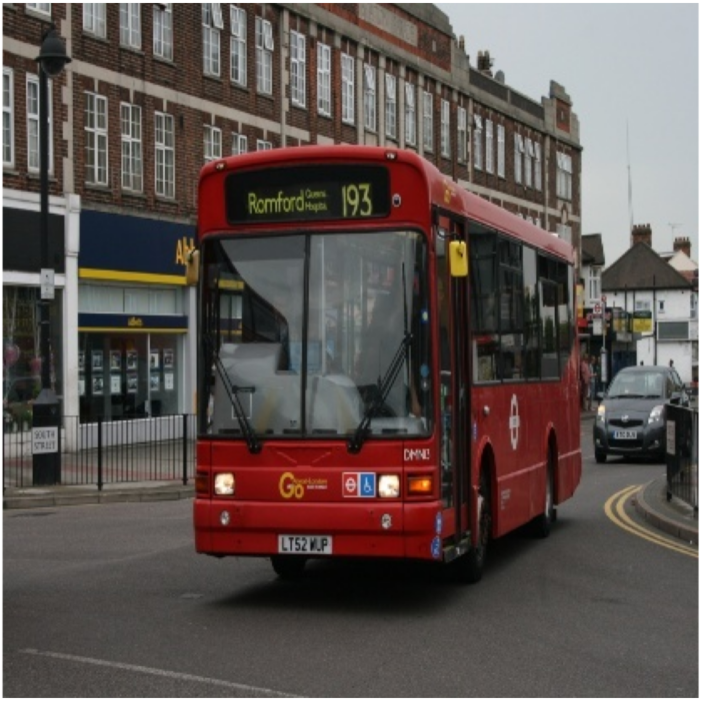
\includegraphics[scale=\scalevaraugmentation]{images/original.png}%
        \label{original}%
        }%
    \hfill%
    \subfloat[Hue]{%
        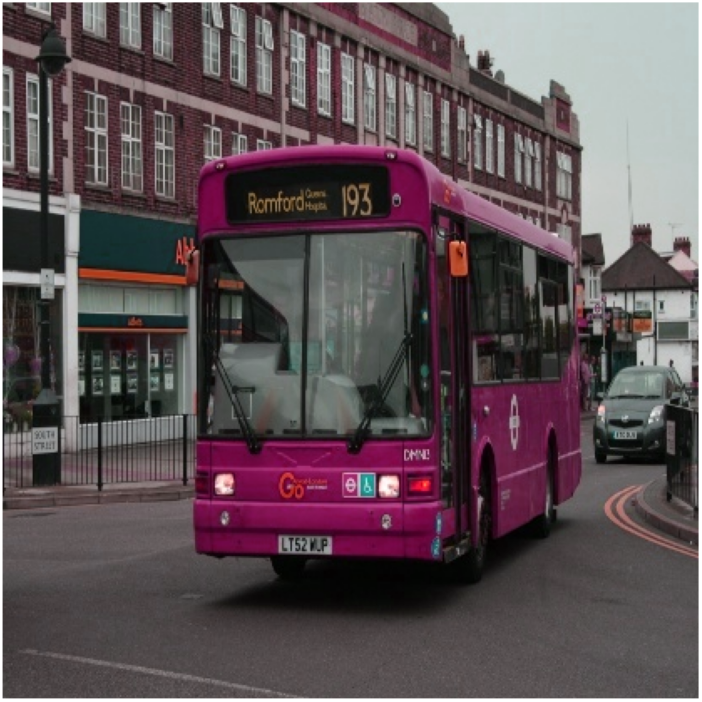
\includegraphics[scale=\scalevaraugmentation]{images/hue.png}%
        \label{hue}%
        }%
    \hfill%
    \subfloat[Brightness]{%
        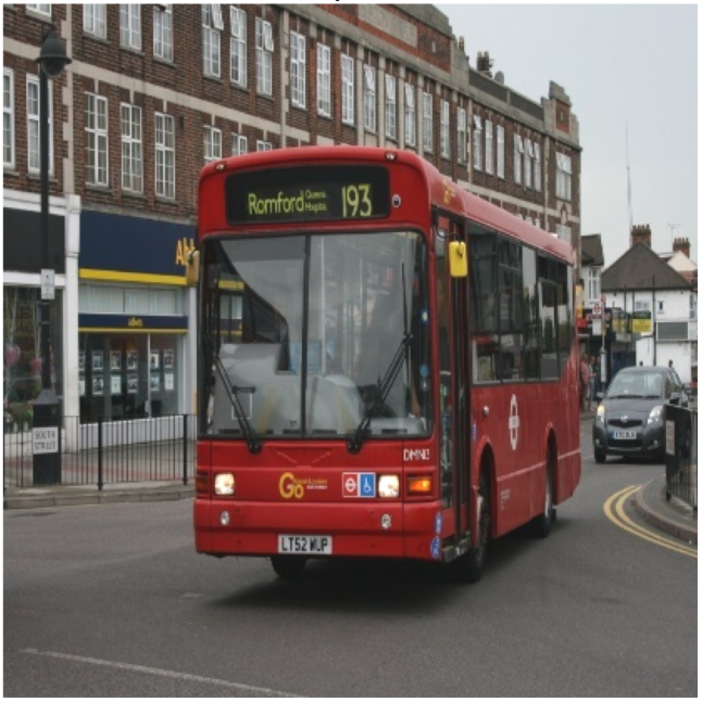
\includegraphics[scale=\scalevaraugmentation]{images/brightness.png}%
        \label{brightness}%
        }%
    \hfill%
    \subfloat[Contrast]{%
        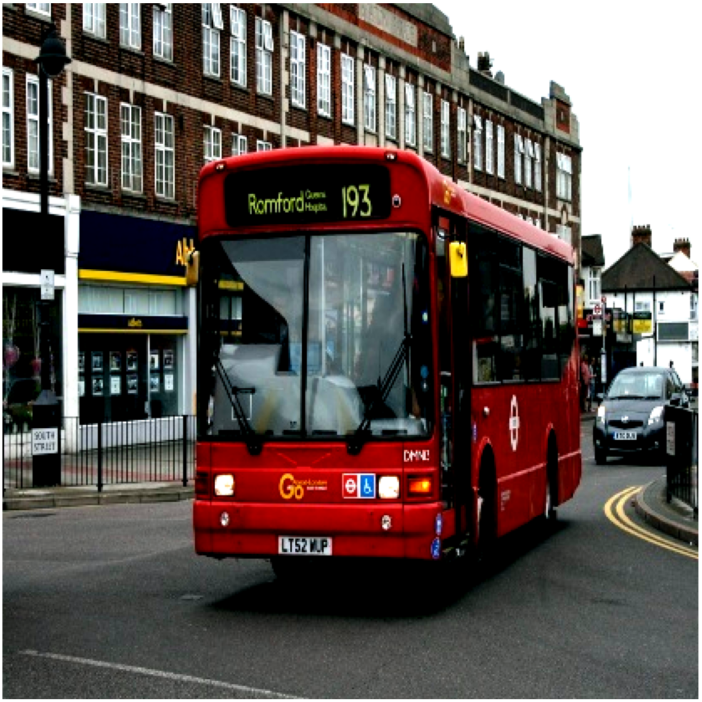
\includegraphics[scale=\scalevaraugmentation]{images/contrast.png}%
        \label{contrast}%
        }%
    \hfill%
    \subfloat[Saturation]{%
        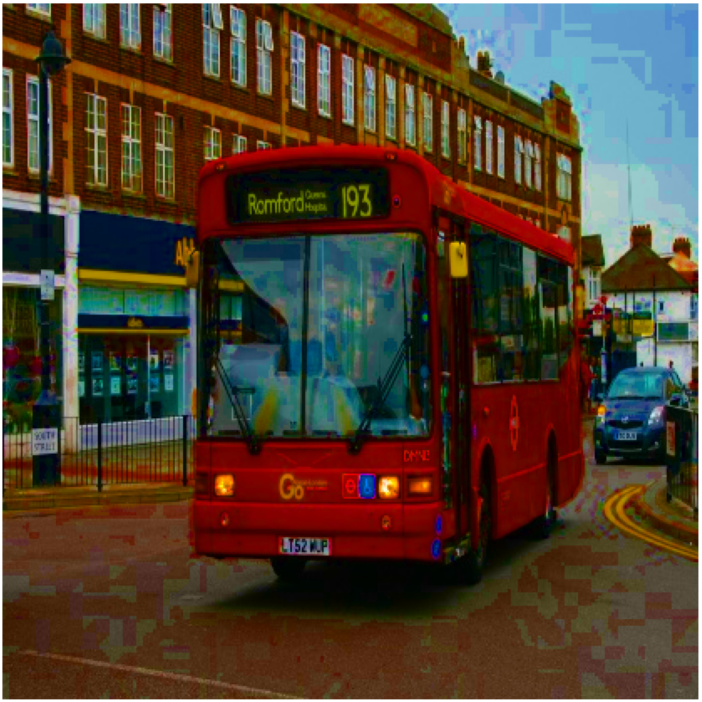
\includegraphics[scale=\scalevaraugmentation]{images/saturation.png}%
        \label{saturation}%
        }%
    \caption{Photometric data augmentation techniques}
    \label{photometric_data_augmentation}
    \end{figure}


    \def \scalevaraugmentationmosaic {0.12}
    \begin{figure}[t] 
    \centering
    \subfloat[Cutout]{%
        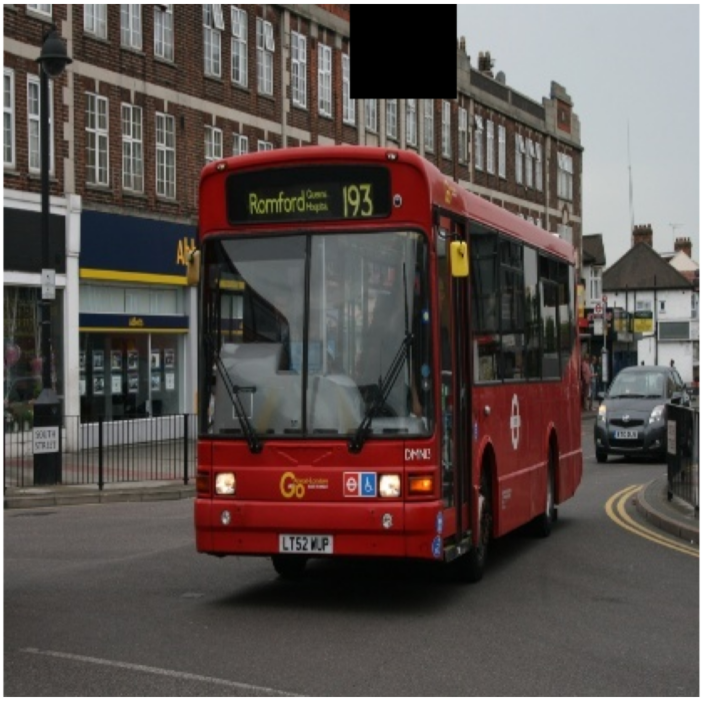
\includegraphics[scale=\scalevaraugmentationmosaic]{images/cutout.png}%
        \label{cutout}%
        }%
    \subfloat[Mosaic]{%
        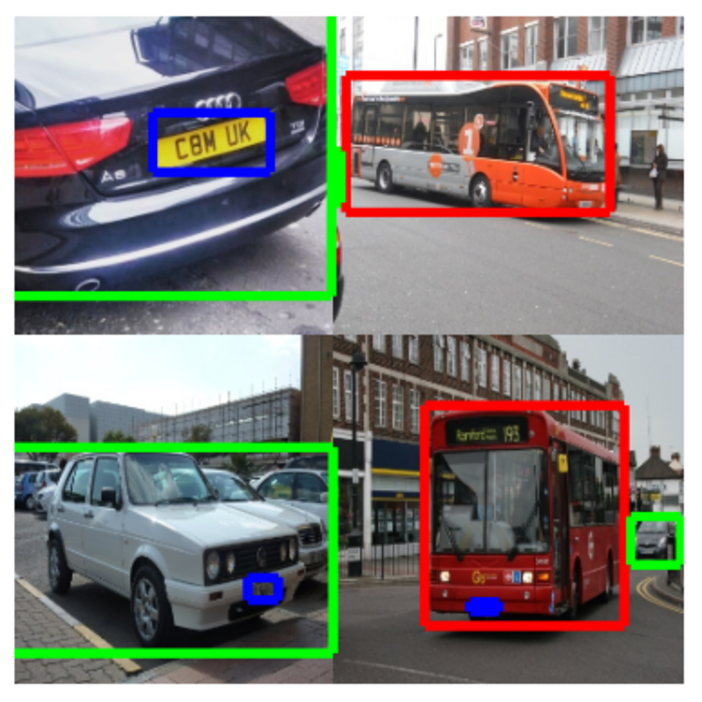
\includegraphics[scale=\scalevaraugmentationmosaic]{images/mosaic.png}%
        \label{mosaic}%
        }%
    \caption{Other data augmentation techniques}
    \label{other_data_augmentation}
    \end{figure}
    
    
    In Fig. \ref{other_data_augmentation} we present other data augmentation techniques that we have used. In Fig. \ref{cutout} we represent the Cutout technique, introduced in \cite{cutout}. The idea is to make the pixels from a random patch in the image black. This way the network should adapt to recognize objects even if they are partially visible. We also follow the recommendation from \cite{cutout}, which states that the patch doesn't have to fit fully in the image. This means that if the center of the patch falls near one of the edges of the image, only the part that overlaps with the images is blacked out.
    
    The other technique is called Mosaic, Fig. \ref{mosaic}, and it was first introduced in \cite{yolov4}. Here, four images are concatenated in order to form a single image. The effect is that the number of bounding boxes in a single image is increased, and the size of the bounding boxes becomes smaller, thus the network should better adapt to small bounding boxes. 

    
    In practice, for each image, we apply a random data augmentation technique from Fig. \ref{photometric_data_augmentation}, and we apply all these data augmentation techniques only during training, and all of them, except Mosaic, are vectorized in order to be computed on the GPU.


